% !TEX encoding = UTF-8 Unicode

\documentclass[a4paper]{article}

\usepackage{color}
\usepackage{url}
\usepackage[utf8]{inputenc}
\usepackage{graphicx}

\usepackage[english,serbian]{babel}

\usepackage[unicode]{hyperref}
\hypersetup{colorlinks,citecolor=green,filecolor=green,linkcolor=blue,urlcolor=blue}

\newtheorem{theorem}{Teorema}[section]

\begin{document}

\title{Sinteza programa\\ \small{Seminarski rad u okviru kursa\\Metodologija stručnog i naučnog rada\\ Matematički fakultet}}

\author{Anja Ivanišević, Ivan Ristović, Milana Kovačević, Vesna Katanić\\ kontakt email prvog, drugog (trećeg) autora}
\date{??.~?? 2018.}
\maketitle

\abstract
U ovom tekstu je ukratko prikazana osnovna forma seminarskog rada. Obratite pažnju da je pored ove .pdf datoteke, u prilogu i odgovarajuća .tex datoteka, kao i .bib datoteka korišćena za generisanje literature. Na prvoj strani seminarskog rada su naslov, apstrakt i sadržaj, i to sve mora da stane na prvu stranu! Kako bi Vaš seminarski zadovoljio standarde i očekivanja, koristite uputstva i materijale sa predavanja na temu pisanja seminarskih radova. Ovo je samo šablon koji se odnosi na fizički izgled seminarskog rada (šablon koji \emph{morate} da ispoštujete!) kao i par tehničkih pomoćnih uputstava. Molim Vas da kada budete predavali seminarski rad, imenujete datoteke tako da sadrže temu seminarskog rada, kao i imena i prezimena članova grupe (ili samo temu i prezimena, ukoliko je sa imenima predugačko). Predaja seminarskih radova biće isključivo preko web forme, a NE slanjem mejla.


\tableofcontents

\newpage


\section{Uvod}
\label{sec:uvod}

Uz sve novouvedene termine u zagradi naglasiti od koje engleske reči termin potiče. Naredni primeri ilustruju način uvođenja enlegskih termina kao i citiranje.

\begin{theorem}
Problem zaustavljanja (eng.~{\em halting problem}) je neodlučiv \cite{haltingproblem}.
\end{theorem}

\begin{theorem}
Za prevođenje programa napisanih u programskom jeziku C može se koristiti GCC kompajler \cite{gcc}.
\end{theorem}

\begin{theorem}
 Da bi se ispitivala ispravost softvera, najpre je potrebno precizno definisati njegovo ponašanje \cite{laski2009software}.
\end{theorem}

Reference koje se koriste u ovom tekstu zadate su u datoteci {\em literature.bib}. Prevođenje u pdf format u Linux okruženju može se uraditi na sledeći način:
\begin{verbatim}
pdflatex TemaImePrezime.tex
bibtex TemaImePrezime.aux
pdflatex TemaImePrezime.tex
pdflatex TemaImePrezime.tex
\end{verbatim}
Prvo latexovanje je neophodno da bi se generisao {\em .aux} fajl. {\em bibtex} proizvodi odgovarajući {\em .bbl} fajl koji se koristi za generisanje literature.
Potrebna su dva prolaza (dva puta pdflatex) da bi se reference ubacile u tekst (tj da ne bi ostali znakovi pitanja umesto referenci). Dodavanjem novih referenci potrebno je ponoviti ceo postupak.


Broj naslova i podnaslova je proizvoljan. Neophodni su samo Uvod i Zaključak. Na poglavlja unutar teksta referisati se po potrebi.
\begin{theorem}
U odeljku \ref{sec:naslov1} precizirani su osnovni pojmovi, dok su zaključci dati u odeljku \ref{sec:zakljucak}.
\end{theorem}

Još jednom da napomenem da nema razloga da pišete:
\begin{verbatim}
\v{s} i \v{c} i \'c ...
\end{verbatim}
Možete koristiti srpska slova
\begin{verbatim}
š i č i ć ...
\end{verbatim}


Ovde pišem uvodni tekst.
Ovde pišem uvodni tekst.
Ovde pišem uvodni tekst.
Ovde pišem uvodni tekst.

\section{Slike i tabele}
\label{slike_i_tabele}

Slike i tabele treba da budu u svom okruženju, sa odgovarajućim naslovima, obeležene labelom da koje omogućava referenciranje.

\begin{theorem} Ovako se ubacuje slika. Obratiti pažnju da je dodato i
\begin{verbatim}
\usepackage{graphicx}
\end{verbatim}

\begin{figure}[h!]
\begin{center}
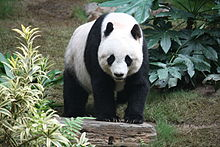
\includegraphics[scale=0.75]{resources/panda.jpg}
\end{center}
\caption{Pande}
\label{fig:pande}
\end{figure}

Na svaku sliku neophodno je referisati se negde u tekstu. Na primer, na slici \ref{fig:pande} prikazane su pande.
\end{theorem}

\begin{theorem} I tabele treba da budu u svom okruženju, i na njih je neophodno referisati se u tekstu. Na primer, u tabeli \ref{tab:tabela1} su prikazana različita poravnanja u tabelama.

\begin{table}[h!]
\begin{center}
\caption{Razlčita poravnanja u okviru iste tabele ne treba koristiti jer su nepregledna.}
\begin{tabular}{|c|l|r|} \hline
centralno poravnanje& levo poravnanje& desno poravnanje\\ \hline
a &b&c\\ \hline
d &e&f\\ \hline
\end{tabular}
\label{tab:tabela1}
\end{center}
\end{table}

\end{theorem}

\section{Prvi naslov}
\label{sec:naslov1}


Ovde pišem tekst.
Ovde pišem tekst.
Ovde pišem tekst.
Ovde pišem tekst.
Ovde pišem tekst.
Ovde pišem tekst.
Ovde pišem tekst.
Ovde pišem tekst.


\subsection{Prvi podnaslov}
\label{subsec:podnaslov1}

Ovde pišem tekst.
Ovde pišem tekst.
Ovde pišem tekst.
Ovde pišem tekst.
Ovde pišem tekst.
Ovde pišem tekst.
Ovde pišem tekst.

\subsection{Drugi podnaslov}
\label{subsec:podnaslov2}

Ovde pišem tekst.
Ovde pišem tekst.
Ovde pišem tekst.
Ovde pišem tekst.
Ovde pišem tekst.
Ovde pišem tekst.

\section{Drugi naslov}
\label{sec:naslov2}

Ovde pišem tekst.
Ovde pišem tekst.
Ovde pišem tekst.
Ovde pišem tekst.

\subsection{... podnaslov}
\label{subsec:podnaslovN}

Ovde pišem tekst.
Ovde pišem tekst.
Ovde pišem tekst.
Ovde pišem tekst.
Ovde pišem tekst.
Ovde pišem tekst.

\section{n-ti naslov}
\label{sec:naslovN}

Ovde pišem tekst.
Ovde pišem tekst.
Ovde pišem tekst.
Ovde pišem tekst.
Ovde pišem tekst.

\subsection{... podnaslov}
\label{subsec:podnaslovK}

Ovde pišem tekst.
Ovde pišem tekst.
Ovde pišem tekst.
Ovde pišem tekst.
Ovde pišem tekst.

\subsection{... podnaslov}
\label{subsec:podnaslovM}

Ovde pišem tekst.
Ovde pišem tekst.
Ovde pišem tekst.
Ovde pišem tekst.
Ovde pišem tekst.

\section{Poslednji naslov}
\label{sec:naslovM}

Ovde pišem tekst.
Ovde pišem tekst.
Ovde pišem tekst.
Ovde pišem tekst.
Ovde pišem tekst.
Ovde pišem tekst.
Ovde pišem tekst.
Ovde pišem tekst.
Ovde pišem tekst.

\section{Zaključak}
\label{sec:zakljucak}

Razvojem tehnika automatske sinteze programa postavlja se pitanje da li će programeri moći da prestanu da govore računarima \textbf{kako} da rade, već da se fokusiraju na to da im kažu \textbf{šta} treba da urade. Ova oblast još uvek nije dovoljno razvijena da bi se koristila za razvijanje realnih, velikih aplikacija. Potrebno je još rada da bi se došlo do toga. Najveći potencijal ima induktivna sinteza programa.
Iako teorijski deluje da ovaj pristup nije dovoljno efikasan, te da će se izvršavati predugo, CEGIS je, kao vodeći predstavnik ove grupe, u praksi pokazao neočekivano dobre rezultate. Uprkos tome, i uspešno sintetisanje manjih programa može značajno da olakša rad programerima. S obzirom na to da najveći deo vremena programeri provedu pišući manje delove koda, pa i automatska sinteza samo tih delova može značajno da ubrza njihov rad.


\addcontentsline{toc}{section}{Literatura}
\appendix
\bibliography{literatura}
\bibliographystyle{plain}

\appendix
\section{Dodatak}
Ovde pišem dodatne stvari, ukoliko za time ima potrebe.
Ovde pišem dodatne stvari, ukoliko za time ima potrebe.
Ovde pišem dodatne stvari, ukoliko za time ima potrebe.
Ovde pišem dodatne stvari, ukoliko za time ima potrebe.
Ovde pišem dodatne stvari, ukoliko za time ima potrebe.


\end{document}
